To fulfil the requirements of the assignment, it is necessary to undertake a comprehensive theoretical analysis of the queueing network.

In order to apply the theoretical notions learned during the course to the estimation of the degree of scalability of the system, the optimal number of users and the identification of the bottleneck of the system, it is first necessary to measure the service times for the queueing network components with regard to the two classes of jobs previously defined.

Although the queries to the endpoint \verb|`/search/:title?page=n'| may vary depending on the parameterization of the URL, we assume that they belong to the same job class.
This assumption will be subsequently confirmed by the empirical results.

\section{Service times measurements}

\subsection{Overview}

Given that we are operating in a ``Processor Sharing'' regime, it is possible for us to exploit the fact that, in the event that there is only one job within the system, its service time is in fact equivalent to the response time.
In light of these considerations, we employed JMeter, a load testing software that will be discussed in greater detail later on, to perform two tests (one for each class of jobs) with the objective of measuring the various service times of our stations.

Both tests comprise a user (a thread) executing a request to the RESTful API at a constant interval of 10 milliseconds.
A total of 10,000 requests are made by the user in both cases, a quantity predetermined by the size of the query set imposed by the assignment.

Details on the tests carried out are provided in the following sections.

\subsection{Test query set}

A Python script was employed to perform a random sampling with reinsertion of 10,000 movie titles based on our MongoDB collections.

It was assumed that the probability of a movie being selected in the extraction is proportional to the number of votes it received.
In order to obtain the most comprehensive query set possible, it was decided to include all movies, all episodes, and all the various linguistic declinations of these in the extraction.
The entire process was carried out using the \verb|pandas.DataFrame.sample| function.

\subsection{RESTful API Profiling}

To obtain the most precise measurement of service times for the two classes of jobs, two different versions of the backend were implemented.
One was employed for load testing and the other was used for the current employment; the latter version contained mechanisms to perform profiling on its execution.

Indeed, within the API, it was necessary to distinguish between the processing times of code in Node.js and those of database aggregation pipelines.
To perform profiling on the Express execution, it was decided to utilise the \verb|PerformanceObserver| Node interface, which forms part of the Performance Timing API.
Indeed, this interface enabled the effective measurement of execution times without the addition of overheads through the utilisation of the \verb|Marks|, namely high-resolution timestamps.

Conversely, regarding MongoDB profiling, the situation was more intricate.
In order to facilitate the process, we proceeded to activate the \verb|system.profile| collection within our database. 
This is a \textit{capped collection}\footnote[1]{A fixed-size collection that performs document insertion and retrieval based on the order in which they were added, exhibiting behaviour analogous to that of circular buffers.} that is created by default by the MongoDB Profiler for each database and hidden from the user.
Its purpose is to measure precise metrics regarding CRUD operations and other administrative and/or configuration commands executed on a running instance of MongoDB.
Consequently, the utilisation of the profiler enabled the accurate determination of the execution times inherent to the aggregation pipelines.

Upon completion of the whole process, all metrics evaluated by the API execution are transcribed asynchronously, thus maintaining optimal performance, by \verb|Pino|.

\verb|Pino.js| is a fast and lightweight Node.js logging library: it is a robust and scalable solution due to its comprehensive asynchronous logging of JSON-formatted files that provides customizable log levels and serializers while maintaining low processing costs.

\subsection{Empirical service times}

Following the execution of the two tests with JMeter, the service times of our system components with respect to the job classes identified in our network are as follows:

\[
\mu^{-1}_{B1} = \num[round-mode=places, round-precision=5]{0.0016899999999999999} \, \text{s}
\quad \quad
\mu^{-1}_{D1} = \num[round-mode=places, round-precision=5]{0.00257625} \, \text{s}
\quad \quad
\mu^{-1}_{B2} = \num[round-mode=places, round-precision=5]{0.00171} \, \text{s}
\quad \quad
\mu^{-1}_{D2} = \num[round-mode=places, round-precision=5]{0.0014637500000000002} \, \text{s}
\]

It should be noted that, although MongoDB employs a scheduling discipline of the ``Processor Sharing'' type, it is not a single-server system analogous to the M/G/1/PS queues analysed during the course.
Consequently, a slight modification was required to the formula for calculating its service times:

\[
	\mu^{-1}_{Dx} = \frac{\overline{R}}{\text{number of CPUs}} \quad \text{where} \quad x \in \{1, 2\}
\]

\section{Bottleneck identification}

Thus far, we have calculated the service times of each station per job class and the relative visit ratios ($\overline{V}_{i}$).
These $\overline{V}_{i}$ are derived from the solutions of the traffic equations and indicate the expected number of visits to each station with respect to each visit made to the reference station (Q\textsubscript{T}).

\[
\overline{V}_{B1} = \num[round-mode=places, round-precision=5]{1.11111111111111}
\quad
\overline{V}_{D1} = \num[round-mode=places, round-precision=5]{1.11111111111111}
\quad
\overline{V}_{B2} = \num[round-mode=places, round-precision=5]{0.888888888888889}
\quad
\overline{V}_{D2} = \num[round-mode=places, round-precision=5]{0.888888888888889}
\quad
\overline{V}_{T} = \num[round-mode=places, round-precision=5]{1.00000000000000}
\]

The data enables the calculation of the service demands ($\overline{D}_i$), which represent the quantity of service requested by a user from each station for each visit to the reference station.
This is achieved through the application of the following formula:

\label{eq:service-demands}
\begin{equation}
	\overline{D}_i = \overline{V}_i \times \mu^{-1}_i \quad \text{where} \quad i \in \{B1, D1, B2, D2\}
\end{equation}

\[
\overline{D}_{B1} = \num[round-mode=places, round-precision=5]{0.00187777777777778}
\quad
\overline{D}_{D1} = \num[round-mode=places, round-precision=5]{0.00286250000000000}
\quad
\overline{D}_{B2} = \num[round-mode=places, round-precision=5]{0.00152000000000000}
\quad
\overline{D}_{D2} = \num[round-mode=places, round-precision=5]{0.00130111111111111}
\]

The results indicate that the database is the bottleneck station. 
A further calculation of the utilisation of each station can be made using the Bottleneck Law:

\label{eq:bottleneck-law}
\begin{equation}
	\rho_i = X_1 \times \overline{D}_i \quad \text{where} \quad i \in \{B1, D1, B2, D2\}
\end{equation}

A graph is provided below, which illustrates the varying levels of station utilisation over the number of users.

\begin{figure}[h]
	\centering
	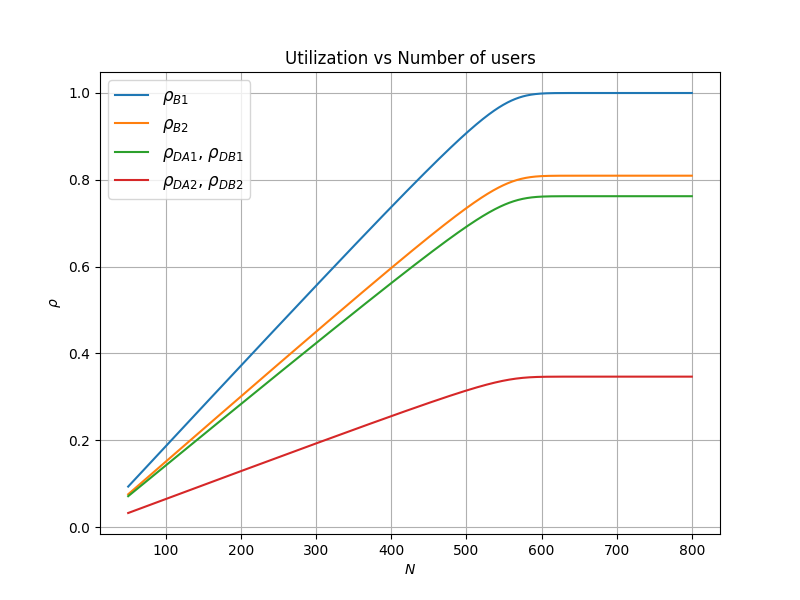
\includegraphics[width=\linewidth]{004/stations-utilization.png}
	\caption{Stations utilisation over the number of users}
\end{figure}

It can be concluded that the database is the component with the highest utilisation rate.

\section{Asymptotic bounds}

In the next section, we will perform a mean value analysis to compute the expected performance indices of our system.
This will be done through Little's Law and the recursive procedure on which this technique is based, without the need to compute the normalization constant G\textsubscript{K} required by Gordon Newell's Theorem.

Prior to conducting the previously announced analysis, a preliminary calculation is conducted using a Python script to determine the upper and lower bounds of response time ($\overline{R}$) and throughput ($X$) in relation to the number of customers in the network.

This is done according to the following formulas:

\label{eq:asymptotic-bounds-expected-response-time}
\begin{equation}
	\overline{R} \geq max\left(\overline{D},N\overline{D}_b-\overline{Z}\right)
\end{equation}

\label{eq:asymptotic-bounds-throughput}
\begin{equation}
	X \leq min\left(\frac{N}{\overline{D}+\overline{Z}},\,\frac{1}{\overline{D}_b}\right) \quad \text{where}
\end{equation}
\[
	\quad \overline{Z} \quad \text{exp. thinking time,} \quad \overline{D}_b \quad \text{bottleneck service demand,} \quad \overline{D} = \sum^{K}_{j=2}\overline{D}_{j}  \\
\]

The parametric values of the calculated limits are provided below:

\[
 R \geq max\left(\num[round-mode=places, round-precision=5]{0.00756138888888889},\;N\times\num[round-mode=places, round-precision=5]{0.00286250000000000}-1\right) \\
\]

\[
 X \leq min\left(\frac{N}{\num[round-mode=places, round-precision=5]{0.00756138888888889}+1},\;\frac{1}{\num[round-mode=places, round-precision=5]{0.00286250000000000}}\right) \\
\]

\section{Mean Value Analysis}

\subsection{JMVA emulation setup}

In order to estimate the performance indices of our queueing network, we employed the ``Java Modelling Tools (JMT)'' suite of applications developed by the ``Politecnico di Milano''.
In particular, we utilised the JMVA (``Mean Value Analysis and Approximate solution algorithms for queueing network models'') application.

The subsequent steps are those required to prepare the emulation within the software according to our queueing network configuration.

\clearpage

1.
The number of customers (50) and the number of classes of jobs were entered.
As can be seen, only one class was indicated, as only class 1 jobs were output from the thinking station.
\begin{figure}[h]
	\centering
	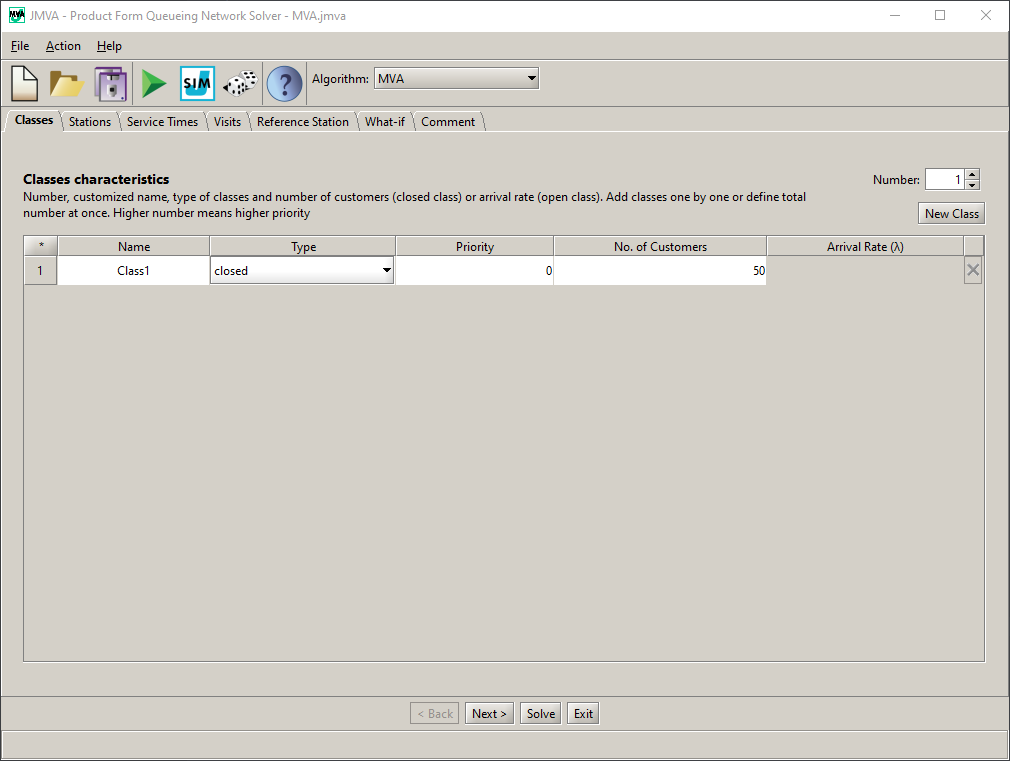
\includegraphics[scale=0.40]{004/JMVA/classes.png}
	\caption{JMVA setup -- classes of jobs}
\end{figure}

2.
The stations in the queueing network are entered according to their respective load type.
The thinking station is designated as a ``delay type'', whereas other stations are classified as ``load-independent'', as their service time remains consistent regardless of the number of customers.
\begin{figure}[h]
	\centering
	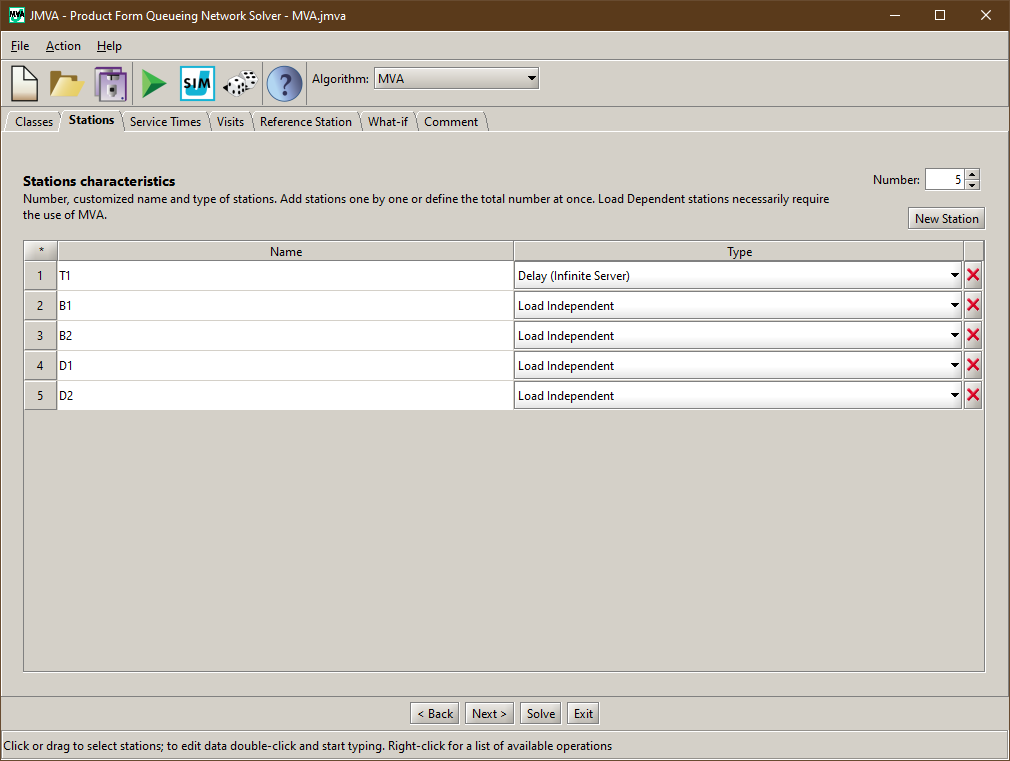
\includegraphics[scale=0.40]{004/JMVA/stations.png}
	\caption{JMVA setup -- stations}
\end{figure}

\clearpage

3.
The service times previously calculated for each station are entered.
\begin{figure}[h]
	\centering
	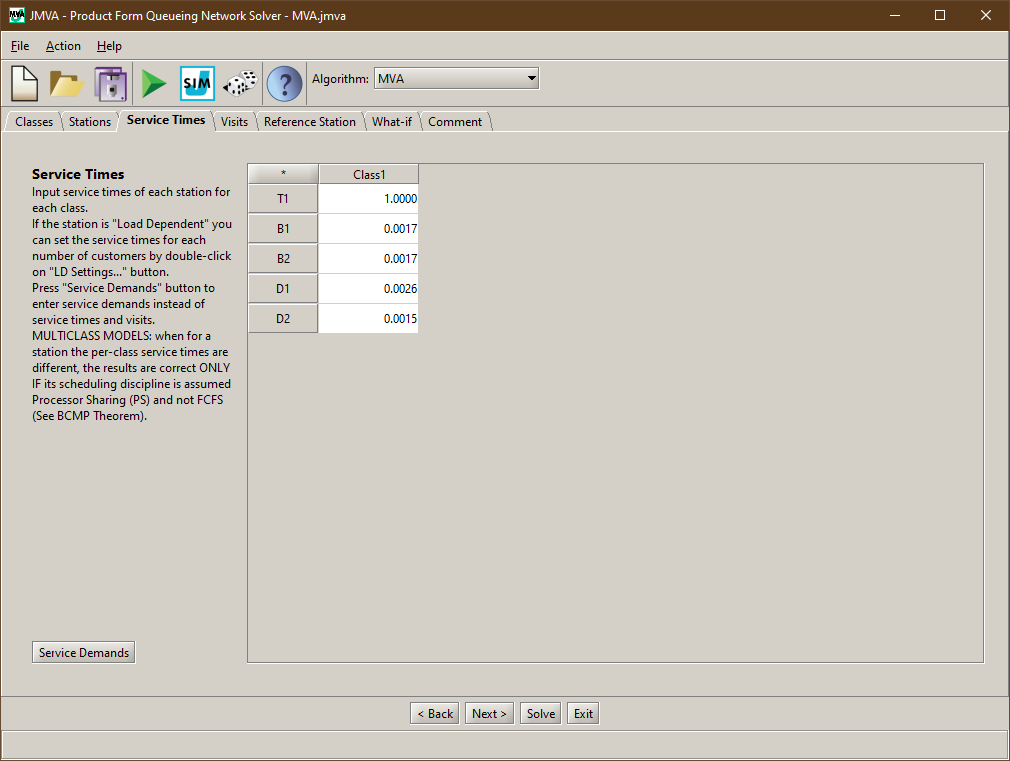
\includegraphics[scale=0.4]{004/JMVA/service_times.png}
	\caption{JMVA setup -- service times}
\end{figure}

4.
The relative visit ratios previously calculated for each station are entered.
\begin{figure}[h]
	\centering
	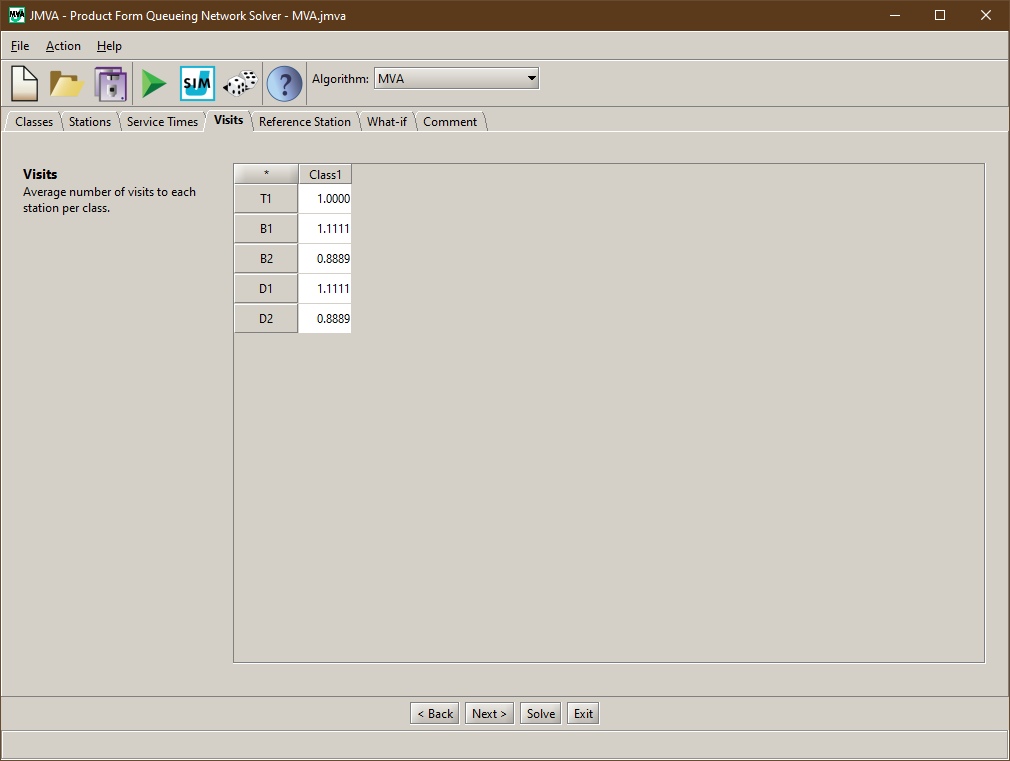
\includegraphics[scale=0.4]{004/JMVA/visits.png}
	\caption{JMVA setup -- relative visit ratios}
\end{figure}

\clearpage

5.
The reference station of the queueing network is indicated.
\begin{figure}[h]
	\centering
	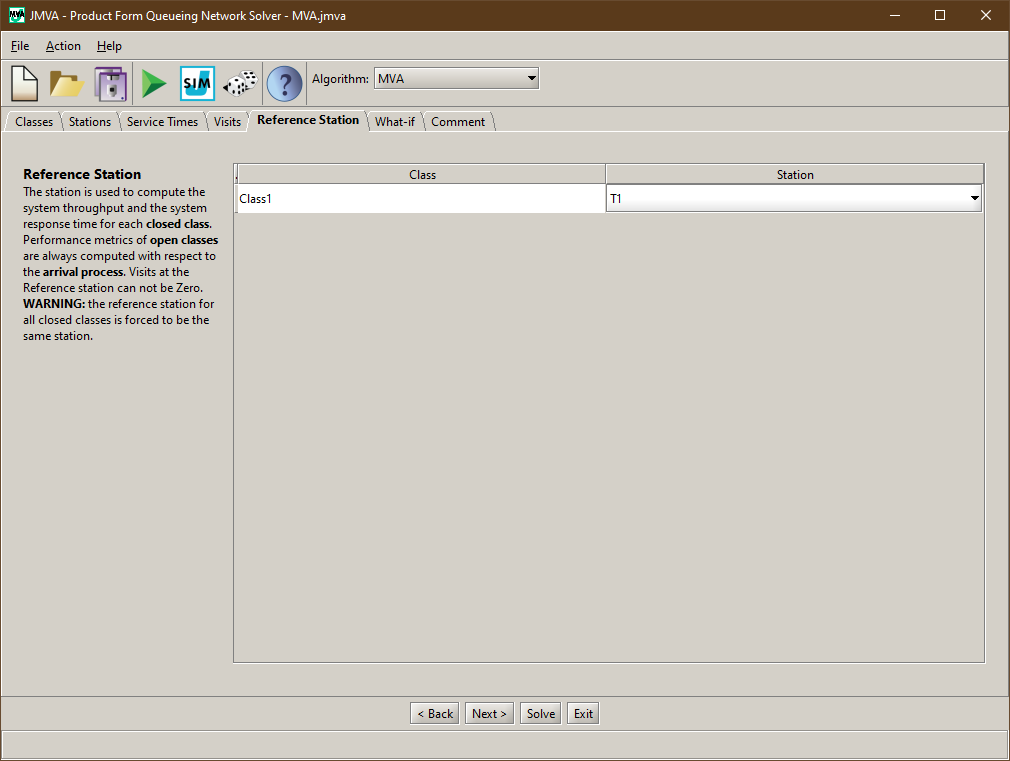
\includegraphics[scale=0.4]{004/JMVA/reference_station.png}
	\caption{JMVA setup -- reference station}
\end{figure}

6.
The initial number of users is indicated as 50, with a subsequent increment of up to 500 users per increment of 1 user.
\begin{figure}[h]
	\centering
	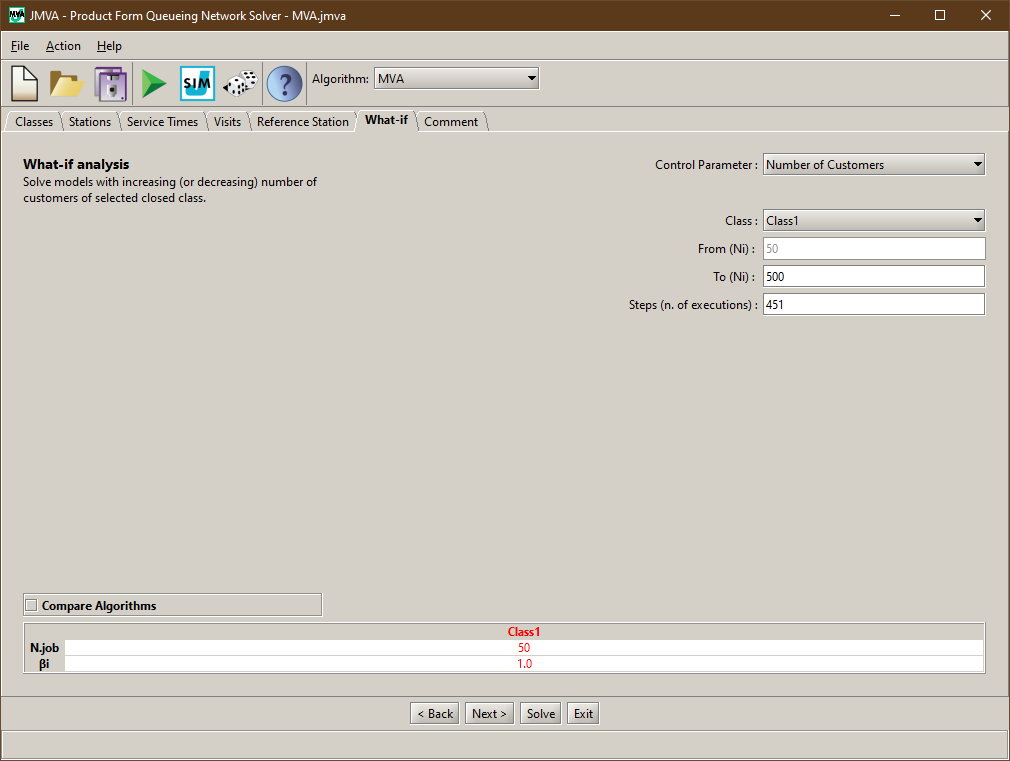
\includegraphics[scale=0.4]{004/JMVA/what_if.png}
	\caption{JMVA setup -- emulation settings}
\end{figure}

\subsection{JMVA emulation results}

The graphs generated by the emulation of JMVA, in conjunction with the previously calculated theoretical bounds, are presented below for the reader's convenience.
As can be observed in the graphs, the optimal number of users has already been determined; this will be calculated in the following section.

\begin{figure}[h]
	\centering
	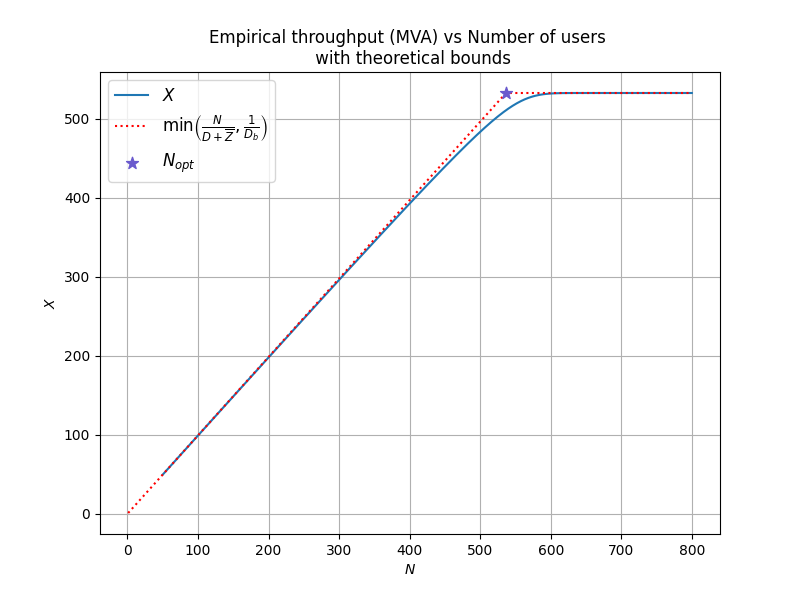
\includegraphics[width=\linewidth]{004/mva-x.png}
	\caption{MVA -- Throughput over the number of users}
\end{figure}

\begin{figure}[h]
	\centering
	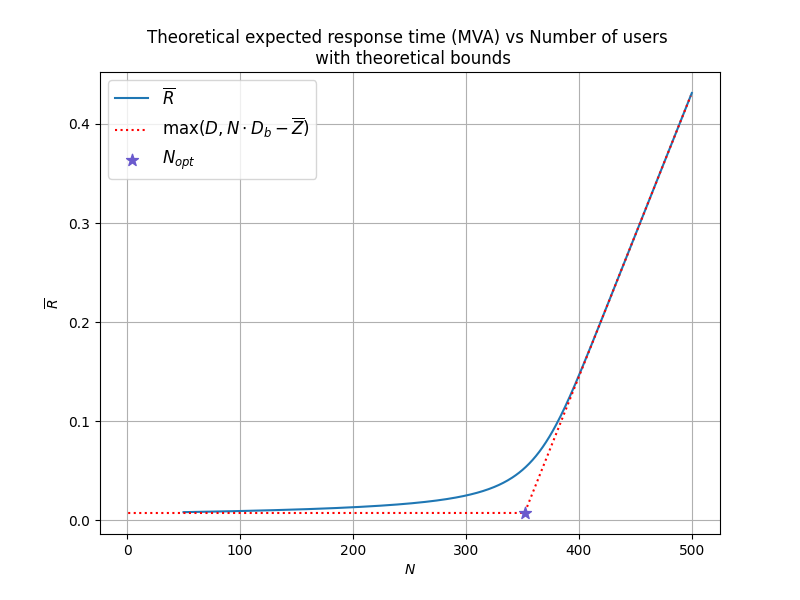
\includegraphics[width=\linewidth]{004/mva-r.png}
	\caption{MVA -- Response time over the number of users}
\end{figure}

\clearpage

\section{Optimal -- theoretical -- number of users}

In conclusion to the theoretical analysis of the queuing network, we proceed with the estimation of the optimal number of users.
This can be obtained from the intersection of the previously calculated asymptotes for throughput and expected response time and with the following formula:

\label{eq:optimal-number-of-users}
\begin{equation}
	N_{opt} = \frac{\overline{D} + \overline{Z}}{\overline{D}_b} = \num[round-mode=places, round-precision=5]{351.986511402232}
\end{equation}

The outcome is fully reflected in the graphs illustrated above.
